\documentclass{article}
\usepackage{assignment_preamble}

\title{Homework 7}
\author{Ravi Kini}
\date{November 30, 2023}

\begin{document}

\maketitle

\problem[\textit{An Introduction to Thermal Physics} (Schroeder, 1e) Exercise 7.6 (extended)]
For a system in thermal and diffusive equilibrium with a reservoir,  the average number of particles in the system $\overline{N}$ is:
\begin{equation}
    \begin{split}
        \frac{k_BT}{\mathcal{Z}}\pderiv{\mathcal{Z}}{\mu} & = \frac{k_BT}{\mathcal{Z}}\pderiv{ }{ \mu}\sum_s e^{-\frac{E\left(s\right) -\mu N\left(s\right)}{k_BT}} \\
        & = \frac{k_BT}{\mathcal{Z}}\sum_s \frac{N(s)}{k_BT} e^{-\frac{E(s) - \mu N(s)}{k_BT}} \\
        & = \sum_s N\left(s\right) \frac{1}{\mathcal{Z}}e^{-\frac{E\left(s\right) - \mu N\left(s\right)}{k_BT}} \\
        & = \sum_s N\left(s\right)\mathcal{P}\left(s\right) = \overline{N} \\
    \end{split}
\end{equation}
The mean square number of particles $\overline{N^2}$ is then:
\begin{equation}
    \begin{split}
        \frac{{\left(k_BT\right)}^2}{\mathcal{Z}}\pderiv{2}{\mathcal{Z}}{\mu^2} & = \frac{{\left(k_BT\right)}^2}{\mathcal{Z}}\pderiv{2}{\mathcal{Z}}{\mu^2}\sum_s e^{-\frac{E\left(s\right) -\mu N\left(s\right)}{k_BT}} \\
        & = \frac{{\left(k_BT\right)}^2}{\mathcal{Z}}\sum_s {\left(\frac{N(s)}{k_BT}\right)}^2 e^{-\frac{E\left(s\right) - \mu N\left(s\right)}{k_BT}} \\
        & = \sum_s N\left(s\right)^2 \frac{1}{\mathcal{Z}}e^{-\frac{E\left(s\right) - \mu N\left(s\right)}{k_BT}} \\
        & = \sum_s N\left(s\right)^2\mathcal{P}\left(s\right) = \overline{N^2} \\
    \end{split}
\end{equation}
The standard deviation $\sigma_N$ is then:
\begin{equation}
    \begin{split}
        \overline{N^2} & = \frac{{\left(k_BT\right)}^2}{\mathcal{Z}}\pderiv{2}{\mathcal{Z}}{ \mu^2} \\
        & = \frac{{\left(k_BT\right)}^2}{\mathcal{Z}}\pderiv{ }{ \mu}\frac{\overline{N}\mathcal{Z}}{k_BT} \\
        & = \frac{k_BT}{\mathcal{Z}}\left(\pderiv{ \overline{N}}{ \mu}\mathcal{Z} + \pderiv{\mathcal{Z}}{ \mu}\overline{N}\right) \\
        & = k_BT\pderiv{ \overline{N}}{ \mu} + \overline{N}^2 \\
        \sigma_N & = \sqrt{\overline{N^2} - \overline{N}^2} \\
        & = \sqrt{k_BT\pderiv{ \overline{N}}{ \mu}}
    \end{split}
\end{equation}
For an ideal gas:
\begin{equation}
    \begin{split}
        \mu & = -k_BT\ln\frac{VZ_{int}}{Nv_Q} \\
        \pderiv{ \mu}{ N} & = -k_BT\ln\frac{VZ_{int}}{Nv_Q} = \frac{k_BT}{N} \\
        \sigma_N & = \sqrt{k_BT\pderiv{ \overline{N}}{ \mu}} \\
        & = \sqrt{k_BT\frac{\overline{N}}{k_BT}} = \sqrt{\overline{N}}
    \end{split}
\end{equation}
For one mole of gas, $\sigma_N \approx 10^{12}$ particles, and $\frac{\sigma_N}{N} \approx 10^{-12}$. The variation is then very negligible.

\clearpage

\problem[\textit{An Introduction to Thermal Physics} (Schroeder, 1e) Exercise 7.7]
The grand free energy $\Phi$ obeys the partial differential equation: 
\begin{equation}
    \begin{split}
        \Phi & = U - TS - \mu N \\
        {\left(\pderiv{ \Phi}{\mu}\right)}_{V,T} & = -N \\
    \end{split}
\end{equation}
Defining $\tilde{\Phi} = -k_BT\ln\mathcal{Z}$, we see that it follows the same partial differential equation.
\begin{equation}
    \begin{split}
        \tilde{\Phi} & = -k_BT\ln\mathcal{Z} \\
        {\left(\pderiv{ \tilde{\Phi}}{\mu}\right)}_{V,T} & = -\frac{k_BT}{\mathcal{Z}}\pderiv{ \mathcal{Z}}{ \mu} = -\overline{N}
    \end{split}
\end{equation}
For $\mu = 0$:
\begin{equation}
    \begin{split}
        \mathcal{Z} & = \sum_s e^{-\frac{E\left(s\right) - 0 \cdot N\left(s\right)}{k_BT}} \\
        & = \sum_s e^{-\frac{E\left(s\right)}{k_BT}} = Z \\
        \Phi & = U - TS = F \\
        \tilde{\Phi} & = -k_BT\ln\mathcal{Z} \\
        & = -k_BT\ln Z = F
    \end{split}
\end{equation}
Since $\Phi$ and $\tilde{\Phi}$ obey the same partial differential equation and agree at $\mu = 0$, $\Phi = \tilde{\Phi} = -k_BT\ln\mathcal{Z}$ for all $T$.

\clearpage

\problem[\textit{An Introduction to Thermal Physics} (Schroeder, 1e) Exercise 7.11 (partial)]
\subproblem{(a)}
For a system of fermions at room temperature, the probability $\overline{n}$ of a single-particle state with energy $\epsilon = \mu - 0.01~\unit{eV}$ being occupied is:
\begin{equation}
    \begin{split}
        \overline{n}\left(\epsilon = \mu - 0.01~\unit{eV}\right) & = \frac{1}{e^{\frac{-0.01~\unit{eV}}{8.617 \cdot 10^{-5}~\unit{eV\per\kelvin} \cdot 293~\unit{\kelvin}}} + 1} \approx 0.598
    \end{split}
\end{equation}
\subproblem{(b)}
The probability $\overline{n}$ of a single-particle state with energy $\epsilon = \mu$ being occupied is:
\begin{equation}
    \begin{split}
        \overline{n}\left(\epsilon = \mu\right) & = \frac{1}{e^{\frac{0~\unit{eV}}{8.617 \cdot 10^{-5}~\unit{eV\per\kelvin} \cdot 293~\unit{\kelvin}}} + 1} \approx 0.5
    \end{split}
\end{equation}
\subproblem{(c)}
The probability $\overline{n}$ of a single-particle state with energy $\epsilon = \mu + 0.01~\unit{eV}$ being occupied is:
\begin{equation}
    \begin{split}
        \overline{n}\left(\epsilon = \mu - 0.01~\unit{eV}\right) & = \frac{1}{e^{\frac{0.01~\unit{eV}}{8.617 \cdot 10^{-5}~\unit{eV\per\kelvin} \cdot 293~\unit{\kelvin}}} + 1} \approx 0.402
    \end{split}
\end{equation}

\clearpage

\problem[\textit{An Introduction to Thermal Physics} (Schroeder, 1e) Exercise 7.13 (partial)]
\subproblem{(a)}
For a system of bosons at room temperature, the average occupancy $\overline{n}$ of a single-particle state with energy $\epsilon = \mu + 0.001~\unit{eV}$ being occupied is:
\begin{equation}
    \begin{split}
        \overline{n}\left(\epsilon = \mu + 0.001~\unit{eV}\right) & = \frac{1}{e^{\frac{0.001}{8.617 \cdot 10^{-5}~\unit{eV\per\kelvin} \cdot 293~\unit{\kelvin}}} - 1} \approx 24.751 \\
    \end{split}
\end{equation}
The probability $\mathcal{P}$ of the state being occupied by $0, 1, 3$ bosons is:
\begin{equation}
    \begin{split}
        \mathcal{P}\left(0\right) & = {\left(e^{-\frac{0.001~\unit{eV}}{8.617 \cdot 10^{-5} \cdot 293}}\right)}^0\left(1 - e^{-\frac{0.001}{8.617 \cdot 10^{-5} \cdot 293}}\right) \approx 0.039 \\
        \mathcal{P}\left(1\right) & = {\left(e^{-\frac{0.001~\unit{eV}}{8.617 \cdot 10^{-5} \cdot 293}}\right)}^1\left(1 - e^{-\frac{0.001}{8.617 \cdot 10^{-5} \cdot 293}}\right) \approx 0.037 \\
        \mathcal{P}\left(3\right) & = {\left(e^{-\frac{0.001~\unit{eV}}{8.617 \cdot 10^{-5} \cdot 293}}\right)}^3\left(1 - e^{-\frac{0.001}{8.617 \cdot 10^{-5} \cdot 293}}\right) \approx 0.034 \\
    \end{split}
\end{equation}
\subproblem{(b)}
The average occupancy $\overline{n}$ of a single-particle state with energy $\epsilon = \mu + 0.01~\unit{eV}$ being occupied is:
\begin{equation}
    \begin{split}
        \overline{n}\left(\epsilon = \mu + 0.01~\unit{eV}\right) & = \frac{1}{e^{\frac{0.01}{8.617 \cdot 10^{-5}~\unit{eV\per\kelvin} \cdot 293~\unit{\kelvin}}} - 1} \approx 2.058 \\
    \end{split}
\end{equation}
The probability $\mathcal{P}$ of the state being occupied by $0, 1, 3$ bosons is:
\begin{equation}
    \begin{split}
        \mathcal{P}\left(0\right) & = {\left(e^{-\frac{0.01~\unit{eV}}{8.617 \cdot 10^{-5} \cdot 293}}\right)}^0\left(1 - e^{-\frac{0.01}{8.617 \cdot 10^{-5} \cdot 293}}\right) \approx 0.327 \\
        \mathcal{P}\left(1\right) & = {\left(e^{-\frac{0.01~\unit{eV}}{8.617 \cdot 10^{-5} \cdot 293}}\right)}^1\left(1 - e^{-\frac{0.01}{8.617 \cdot 10^{-5} \cdot 293}}\right) \approx 0.220 \\
        \mathcal{P}\left(3\right) & = {\left(e^{-\frac{0.01~\unit{eV}}{8.617 \cdot 10^{-5} \cdot 293}}\right)}^3\left(1 - e^{-\frac{0.01}{8.617 \cdot 10^{-5} \cdot 293}}\right) \approx 0.100 \\
    \end{split}
\end{equation}

\clearpage

\problem[\textit{An Introduction to Thermal Physics} (Schroeder, 1e) Exercise 7.18]
For a type of particle that can share a single particle state with up to one other particle, the distribution function $\mathcal{Z}$ is:
\begin{equation}
    \begin{split}
        \mathcal{Z} & = 1 + e^{-\frac{\epsilon - \mu}{k_BT}} + e^{-\frac{2\left(\epsilon - \mu\right)}{k_BT}} \\
        & = 1 + e^{-x} + e^{-2x} \\
        \overline{n} & = -\frac{1}{\mathcal{Z}}\pderiv{\mathcal{Z}}{ x} \\
        & = -\frac{-e^{-x} - 2e^{-2x}}{1 + e^{-x} + e^{-2x}} \\
        & = \frac{e^{-x} + 2e^{-2x}}{1 + e^{-x} + e^{-2x}} \\
    \end{split}
\end{equation}

\begin{center}
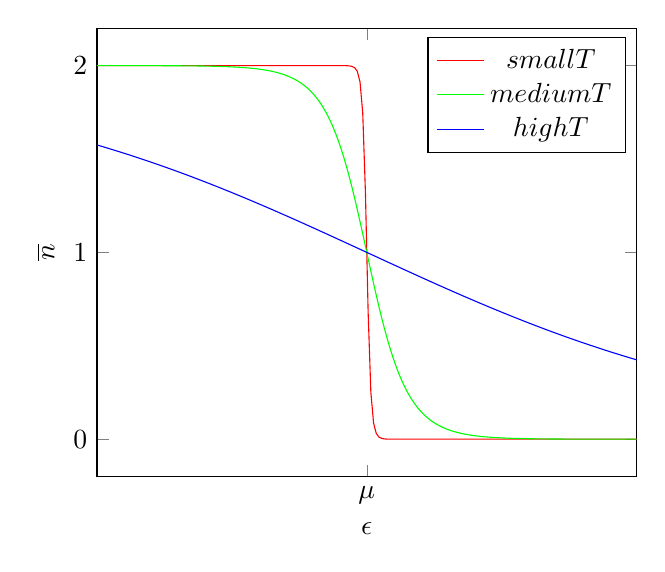
\begin{tikzpicture}
\begin{axis}[samples=200,xlabel=$\epsilon$,ylabel=$\overline{n}$,ytick={0,1,2},xtick={1},xticklabels={$\mu$},xmin=0,xmax=2]
\addplot[color=red,domain=0:2]{(e^(-1 * (x - 1)/0.01) + 2 * e^(-2 * (x - 1)/0.01)) / (1 + e^(-1 * (x - 1)/0.01) + e^(-2 * (x - 1)/0.01))};
\addlegendentry{$\text{small }T$}
\addplot[color=green,domain=0:2]{(e^(-1 * (x - 1)/0.1) + 2 * e^(-2 * (x - 1)/0.1)) / (1 + e^(-1 * (x - 1)/0.1) + e^(-2 * (x - 1)/0.1))};
\addlegendentry{$\text{medium }T$}
\addplot[color=blue,domain=0:2]{(e^(-1 * (x - 1)/1) + 2 * e^(-2 * (x - 1)/1)) / (1 + e^(-1 * (x - 1)/1) + e^(-2 * (x - 1)/1))};
\addlegendentry{$\text{high }T$}
\end{axis}
\end{tikzpicture}
\end{center}

\clearpage

\problem[\textit{An Introduction to Thermal Physics} (Schroeder, 1e) Exercise 7.19 (partial)]
The Fermi energy $\epsilon_F$ and Fermi temperature $T_F$ are:
\begin{equation}
    \begin{split}
        \epsilon_F & = \frac{h^2}{8m}{\left(\frac{3}{\pi}\frac{N}{V}\right)}^{\frac{2}{3}} \\
        & = \frac{{\left(6.626 \cdot 10^{-34}~\unit{\joule\second}\right)}^2}{8 \cdot 9.11 \cdot 10^{-31}~\unit{\kilogram}}{\left(\frac{3}{\pi}\cdot 8.5 \cdot 10^{28}~\unit{\per\meter\cubed}\right)}^{\frac{2}{3}} \\
        & \approx 1.129 \cdot 10^{-18}~\unit{\joule} \approx 7.049~\unit{eV} \\
        T_F & = \frac{\epsilon_F}{k_B} \\
        & = \frac{1.129 \cdot 10^{-18}~\unit{\joule}}{1.381 \cdot 10^{-23}~\unit{\joule\per\kelvin}} \approx 81776~\unit{\kelvin}
    \end{split}
\end{equation}
Room temperature is sufficiently low to treat this system as a degenerate Fermi gas.

\clearpage

\problem[\textit{An Introduction to Thermal Physics} (Schroeder, 1e) Exercise 7.23 (partial)]
\subproblem{(a)}
The total kinetic energy of the degenerate electrons $U_{\text{kinetic}}$ is:
\begin{equation}
    \begin{split}
        U_{\text{kinetic}} & = \frac{3}{5}N\epsilon_F \\
        & = \frac{3}{5}N\frac{h^2}{8m_e}(\frac{3}{\pi}\frac{N}{V})^{\frac{2}{3}} \\
        & = \frac{3}{5}(\frac{M}{2m_p})\frac{h^2}{8m_e}(\frac{3}{\pi}\frac{\frac{M}{2m_p}}{\frac{4}{3}\pi R^3})^{\frac{2}{3}} \\
        & = \frac{3}{80}(\frac{9}{8\pi^2})^{\frac{2}{3}}\frac{h^2M^{\frac{5}{3}}}{m_em_p^{\frac{5}{3}}R^2} \\
        & \approx 0.0088\frac{h^2M^{\frac{5}{3}}}{m_em_p^{\frac{5}{3}}R^2} \\
    \end{split}
\end{equation}
\subproblem{(b)}
\begin{center}
\begin{tikzpicture}
\begin{axis}[samples=200,xlabel=$R$,ylabel=$U_{\text{kinetic}} + U_{\text{grav}}$,ytick={0},xtick={0},xticklabels={},xmin=0,xmax=3]
\addplot[color=red,domain=0.9:3]{1/x^2 - 1/x};
\end{axis}
\end{tikzpicture}
\end{center}

The equilibrium radius $R'$ is:
\begin{equation}
    \begin{split}
        U & = U_{\text{kinetic}} + U_{\text{grav}} \\
        & = 0.0088\frac{h^2M^{\frac{5}{3}}}{m_em_p^{\frac{5}{3}}R^2} - \frac{3}{5}\frac{GM^2}{R} \\
        \left.\frac{dU}{dR}\right\vert_{R'} = 0 & = -2 \cdot 0.0088\frac{h^2M^{\frac{5}{3}}}{m_em_p^{\frac{5}{3}}R'^3} + \frac{3}{5}\frac{GM^2}{R'^2} \\
        & = \frac{1}{R'^2}(-2 \cdot 0.0088\frac{h^2M^{\frac{5}{3}}}{m_em_p^{\frac{5}{3}}R'} + \frac{3}{5}GM^2)\\
        R' & = \frac{2 \cdot 0.0088\frac{h^2M^{\frac{5}{3}}}{m_em_p^{\frac{5}{3}}}}{\frac{3}{5}GM^2} \\
        & \approx 0.0293\frac{h^2}{Gm_em_p^{\frac{5}{3}}}M^{-\frac{1}{3}}
    \end{split}
\end{equation}
As mass increases, radius decreases. This makes sense, as increasing mass increases the gravitational attraction of the white dwarf. Consequently, the white dwarf contracts, so the decrease in the gravitational potential energy is greater than the increase in kinetic energy.
\subproblem{(c)}
For $M = 2 \cdot 10^{30}~\unit{\kilo\gram}$, the equilibrium radius $R'$ and density $\rho$ are:
\begin{equation}
    \begin{split}
        R' & = 0.0293\frac{h^2}{Gm_em_p^{\frac{5}{3}}}{\left(2 \cdot 10^{30}~\unit{\kilo\gram}\right)}^{-\frac{1}{3}} \\
        & \approx 7.134 \cdot 10^{6}~\unit{\meter} \approx 7134~\unit{\kilo\meter} \\
        \rho = \frac{M}{\frac{4}{3}\pi R'^3} & = \frac{2 \cdot 10^{30}~\unit{\kilo\gram}}{\frac{4}{3}\pi \cdot {\left(7.134 \cdot 10^{6}~\unit{\meter}\right)}^3} \\
        & \approx 1.315 \cdot 10^9~\unit{\frac{\kilo\gram}{\meter\cubed}}
    \end{split}
\end{equation}
The density is over a million times the density of water.
\subproblem{(d)}
The Fermi energy $\epsilon_F$ and Fermi temperature $T_F$ are:
\begin{equation}
    \begin{split}
        \epsilon_F & = \frac{h^2}{8m_e}{\left(\frac{3}{\pi}\frac{N}{V}\right)}^{\frac{2}{3}} \\
        & = \frac{h^2}{8m_e}{\left(\frac{3}{\pi}\frac{\frac{M}{2m_p}}{\frac{4}{3}\pi R^3}\right)}^{\frac{2}{3}} \\
        & = \frac{h^2}{8m_e}{\left(\frac{3}{\pi}\frac{\frac{2 \cdot 10^{30}~\unit{\kilo\gram}}{2m_p}}{\frac{4}{3}\pi {\left(7.134 \cdot 10^6~\unit{\meter}\right)}^3}\right)}^{\frac{2}{3}} \\
        & \approx 3.135 \cdot 10^{-14}~\unit{\joule} \approx 1.957 \cdot 10^5 ~\unit{eV} \\
        T_F & = \frac{\epsilon_F}{k_B} \\
        & = \frac{3.135 \cdot 10^{-14}~\unit{\joule}}{1.381 \cdot 10^{-23}~\unit{\joule\per\kelvin}} \approx 2.270 \cdot 10^9~\unit{\kelvin}
    \end{split}
\end{equation}
The Fermi temperature is several times hotter than the sun, and likely any white dwarf, so $T \approx 0$ and the system can be treated as a degenerate Fermi gas.

\end{document}